



\documentclass[a4paper,12pt,spanish]{article}

\usepackage[utf8]{inputenc}


\usepackage{blindtext}
%\usepackage{microtype}
\usepackage{amsfonts, amsmath, amsthm, amssymb}
%\usepackage{fancyhdr}
%\usepackage{index}
%\usepackage{multicol}    

%\usepackage{booktabs}

\usepackage[T1]{fontenc}
\usepackage[utf8]{inputenc}
\usepackage{graphicx}
\usepackage[spanish,es-tabla]{babel}
\usepackage{url}
\usepackage{enumitem}

\usepackage[unicode=true, pdfusetitle,
bookmarks=true,bookmarksnumbered=false,bookmarksopen=false,
breaklinks=true,pdfborder={0 0 1},backref=false,colorlinks=false]
{hyperref}

\usepackage{listings}
\usepackage{longtable}


\usepackage{siunitx} %para el sistema internacional
\usepackage[export]{adjustbox}
\usepackage{booktabs} 
\usepackage{subcaption}

\usepackage{float}


\newcommand{\address}[1]{
	\par {\raggedright #1
		\vspace{1.4em}
		\noindent\par}
}

\usepackage[table,xcdraw]{xcolor}


\pagenumbering{gobble}
\include{noNumberPage}
\pagenumbering{arabic}
\setcounter{page}{1}

%tutorial de tablas latex: https://manualdelatex.com/tutoriales/tablas

\usepackage{multirow}

% \usepackage[table,xcdraw]{xcolor}


%Inicio del documento (hasta que se cierre con \end{document}
\begin{document}
	
	
	\title{Caracterización de un Contador Geiger-Müller}
	
	%\author{Adrián Rivero Fernández}
	\date{}
	
	\maketitle
	
	
	
	
	
	
	
	
	
	\iffalse %comentarios de varias líneas con un if, poner en true si queremos que suceda
	\begin{abstract} %resumen
		
		
		Pretendemos estudiar la conservación de la energía mecánica de un sólido con rotación y desplazamiento, y la determinación del momento de inercia de la rueda de Maxwell.
		
	1. Determinación de la curva característica con la meseta o ?uuuuuuuuplateau? del con-
	tador y de su pendiente. Tensión umbral y tensión de operación.
	2. Obtención del tiempo de resolución (Método de la dos fuentes).
	3. Determinación de la eficiencia del detector, con muestras calibradas.
		
		
	\end{abstract} 
	\fi
	
\iffalse
I don't want this to happen
\fi


	
	\section{Objetivos de la práctica}
	
	\vspace{\baselineskip}
	
	1. Determinar la curva característica con la meseta o "plateau" del contador y de su pendiente. Tensión umbral y tensión de operación.\\
	
	2. Obtener el tiempo de resolución.\\
	
	3. Determinar la eficiencia del detector, con muestras calibradas.\\
	
	
	\iffalse
	\section{Introducción}
	
	El detector de Geiger-Müller es un cilindro con una mezcla de gases (argón y helio generalmente). Tiene un hilo conductor fino a lo largo de su eje, el cual actúa de ánodo en un sistema de recogida de carga cuando se aplica una tensión V entre el hilo y la pared, que actúa de cátodo.
	
	
	
	
	
	
	En un detector gaseoso de ionización ideal, cuando una partícula cargada penetra en el interior, crea pares iónicos que, al aplicar un campo eléctrico entre cátodo y ánodo, acelerará las cargas positivas hacia el cátodo y las negativas hacia el ánodo. Si el campo	eléctrico es pequeño, algunos pares iónicos se recombinan entre sí antes de llegar al electrodo, y por lo tanto la carga recogida será menor de lo que debería. 
	
	Al aumentar el campo eléctrico, todos los pares iónicos llegarían a los electrodos.
	Al aumentar la tensión, los iones formados adquirirían suficiente energía como para producir a su vez nuevos iones, fenómeno que se conoce como \textbf{ionización secundaria}. La carga recogida sería mayor que la inicial, pero proporcional a ella según un factor llamado \textbf{factor de amplificación}.
	
	Al seguir aumentando la tensión aumenta este factor, hasta que la ionización secundaria es tan grande que crea un campo repulsivo en las proximidades de los
	electrodos, y la carga acumulada ya no sería proporcional a la incidente.
	
	Al crecer más, el campo la carga recogida aumenta con el voltaje aplicado y la descarga se extiende a todo el volumen del contador. Es independiente de la ionización inicial y la energía producida por la partícula. 
	Esta es la región en la que trabaja el detector Geiger. Con un nuevo aumento de la tensión, la avalancha de electrones secundarios produce una descarga continua. Para extiguirla se suele introducir en el gas trazas de algún halógeno, Cl o Br, de forma que neutralicen parte de los iones.
	
	
	
	
	\section{Instrumentación}
	
	El detector Geiger está cubierto con un blindaje de plomo para disminuir la	radiación de fondo. El castillete de blindaje permite colocar la fuente radiactiva a distintas alturas. El flujo de partículas incidente penetrará en el interior del detector a través de una ventana de mica, y el campo eléctrico entre los electrodos se aplicará mediante una fuente de alta tensión (de hasta 1.000 V).
	
	Existe un fondo de radiación por rayos cósmicos, radiación natural de elementos en paredes y ambiente, y ruido electrónico del detector. Este fondo habrá que restarlo en las medidas que tomemos con el detector.
	
	El detector Geiger-Müller es considerado un detector de respuesta rápida a la radiación, debido a su capacidad para amplificar rápidamente las señales de radiación incidente y producir una respuesta eléctrica detectable. Esta característica lo hace ideal para tareas como la monitorización de radiación ambiental o la detección de material radiactivo, pero presenta una menor capacidad para diferenciar distintos tipos de radiación y presenta saturación en altas tasas de conteo.
	

	
	
	
	
	\iffalse
	
	\section{Determinación del fondo}
	
	Existe un fondo de radiación por rayos cósmicos, radiación natural de elementos en paredes y ambiente, y ruido electrónico del detector. Este fondo habrá que restarlo en las medidas que tomemos con el detector.
	
	% Please add the following required packages to your document preamble:
	% \usepackage{multirow}
	\begin{table}[H]
		\centering
		\begin{tabular}{|c|l|}
			
			\hline
			\multirow{4}{*}{Medidas}       & 47   \\ \cline{2-2} 
			& 67   \\ \cline{2-2} 
			& 59   \\ \cline{2-2} 
			& 43   \\ \hline\hline
			\multicolumn{1}{|l|}{Promedio} & 54   \\ \hline\hline
			\multicolumn{1}{|l|}{Bq}       & 0,60 \\ \hline
		\end{tabular}
	
	\caption{Fondo}
	\end{table}
	
	\fi
	\fi
	
	\section{Obtención de la curva característica}
	
	La curva característica del detector es una representación de la tasa de cuentas respecto al voltaje aplicado al detector, de modo que podemos ver como se relacionan. Estas curvas presentan tres regiones diferenciadas, como las vistas en la Figura \ref{fig:grafica0}, y nos da información útil sobre cómo ajustar el voltaje para optimizar el rendimiento del detector según la necesidad específica.
	
	\begin{figure}[H]
		\centering
		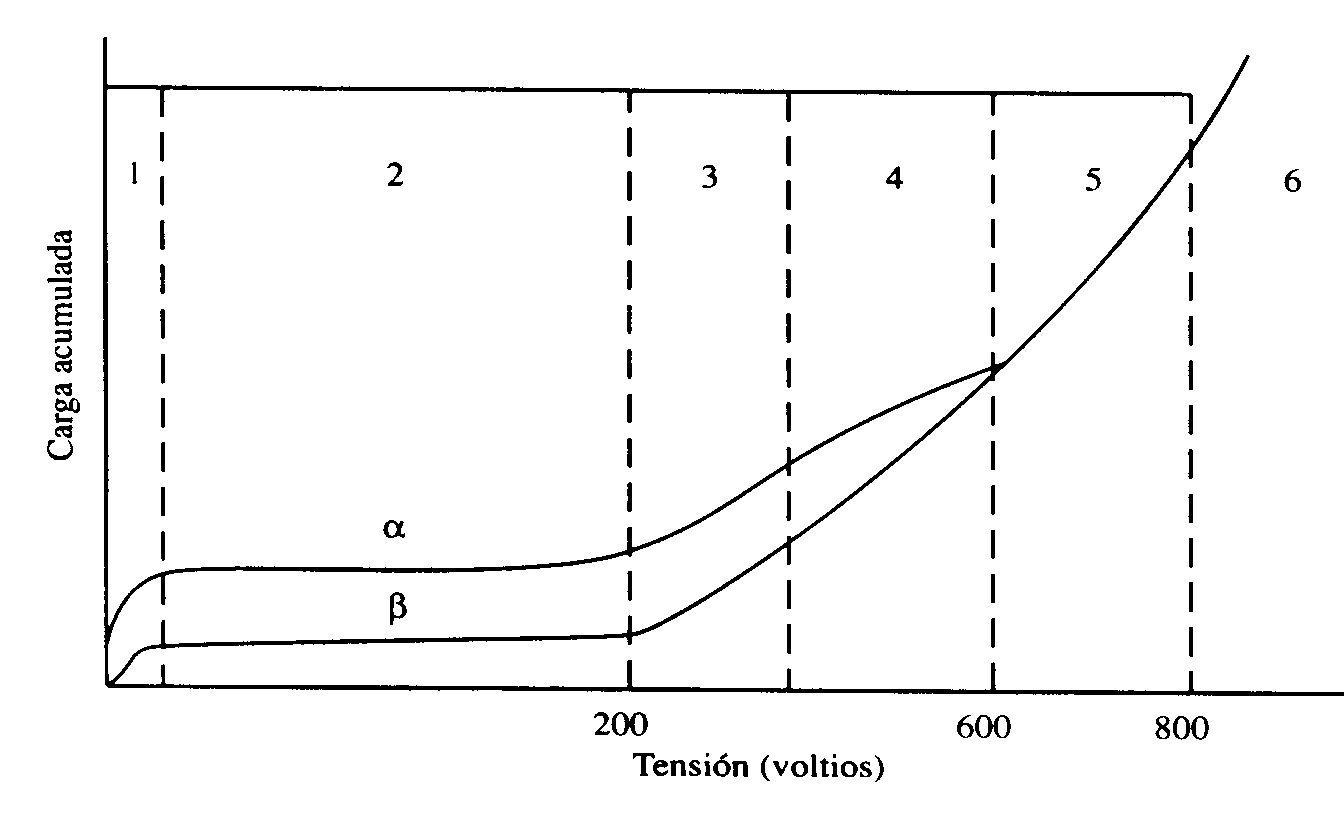
\includegraphics[width=0.6\linewidth]{imagenes/grafica0}
		\caption{Variación de carga frente tensión aplicada en un detector}
		\label{fig:grafica0}
	\end{figure}
	
	
	Para obtener la curva, coloramos la fuente de Co-60 en la bandeja inferior, y tomamos las medidas durante 90s a lo largo de diferentes voltajes. 
	
	
	\begin{table}[H]
		\centering
		\begin{tabular}{|c|c|c|}
			\hline
			Tensión (V) & Cuentas & Bq     \\ \hline
			700         & 0       & 0      \\ \hline
			720         & 0       & 0      \\ \hline
			740         & 6       & 0,067  \\ \hline
			760         & 5049    & 56,1   \\ \hline
			780         & 5173    & 57,478 \\ \hline
			800         & 5283    & 58,7   \\ \hline
			820         & 5347    & 59,412 \\ \hline
			840         & 5500    & 61,111 \\ \hline
			860         & 5689    & 63,211 \\ \hline
			880         & 5817    & 64,633 \\ \hline
		\end{tabular}
		\caption{Datos para la curva característica}
		\label{tab:my-table}
	\end{table}
	
	
	\begin{figure}[H]
		\centering
		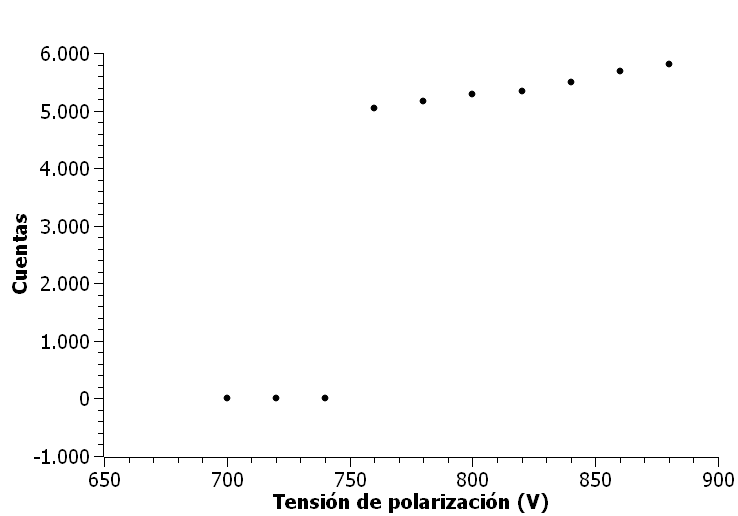
\includegraphics[width=1\linewidth]{imagenes/curva-caracteristica-cuentas-tension}
		\caption{Curva característica}
		\label{fig:curva-caracteristica-cuentas-tension}
	\end{figure}
	
	Podemos ver en la Figura \ref{fig:curva-caracteristica-cuentas-tension} que se diferencian dos de las tres zonas de la curva característica. Partiendo de la condición inicial en la que no detecta nada, hay una zona en la que la radiación aumenta, hasta llegar a la meseta. \\
	
	
	Se comienza a detectar actividad en la tensión umbral 
	\[V_u = 760  \si{V}  \]
	
	
	La meseta llega desde esta tensión umbral hasta nuestra medida de mayor valor, por lo que 
	\[V_f - V_i = 880 - 720 = 160 \si{V}\]
	
	Como la longitud de la meseta es inferior a 200V, aunque cercana, la tensión de trabajo
	\[V_{trabajo} = 820\si{V}\]
	
	La pendiente relativa al punto medio queda 
	\[ \text{P} = \frac{(R_f- R_i)/[(R_f-R_i)/2]}{(V_f - V_i)/100} \times 100 = 11,78 \text{(\% 100V)}
	\]
	
	Un buen detector puede tener una pendiente del 2-3\%. Nuestro detector lo sobrepasa, debido bien al desgaste, al diseño o a la calibración.\\
	
	A continuación, vendría un aumento de la carga, pero nuestro aparato aguanta un máximo de 880V por lo que no podemos tratar de medirla. 
	
	\section{Tiempo muerto y tiempo de resolución}
	
	El detector Geiger-Müller es considerado un detector de respuesta rápida a la radiación, debido a su capacidad para amplificar rápidamente las señales de radiación incidente y producir una respuesta eléctrica detectable. \\
	
	Debido al campo repulsivo por la ionización que produce la primera partícula en torno a los electrodos del detector, este no puede detectar una segunda hasta pasado cierto tiempo (alrededor de 100$\mu$s). A este tiempo se le llama \textbf{tiempo muerto} ($t_m$). \\
	Es posible que la amplitud del segundo impulso sea menor que el primero y no se detecte en la unidad de recuento. Al tiempo hasta que se detecte otro impulso se llama tiempo de resolución $\tau_r$.\\
	
	Pasado cierto tiempo de recuperación $t_r$ se igualan las amplitudes del detector y del impulso inicial.\\
	
	
	Para calcular el tiempo de resolución, que para una sensibilidad fija del receptor será lo mismo que el tiempo muerto, utilizaremos el método de las dos fuentes, mediante el que tomaremos datos de distintas fuentes por separado y en conjunto para deducir el tiempo de resolución mediante la expresión. En este punto es importante que la posición de estas fuentes sea la misma para cada una cuando están separadas que cuando están juntas, ya que la geometría y posición en relación al punto de detección afectará a la cantidad de partículas detectadas. 
	
	\[ \tau_r = \frac{A'_{12}+ F' - A_1'- A'_2}{A'^2_1 + A'^2_2 - F'^2 - A'^2_{12}}
	\]
	
	
	\begin{figure}[]
		\centering
		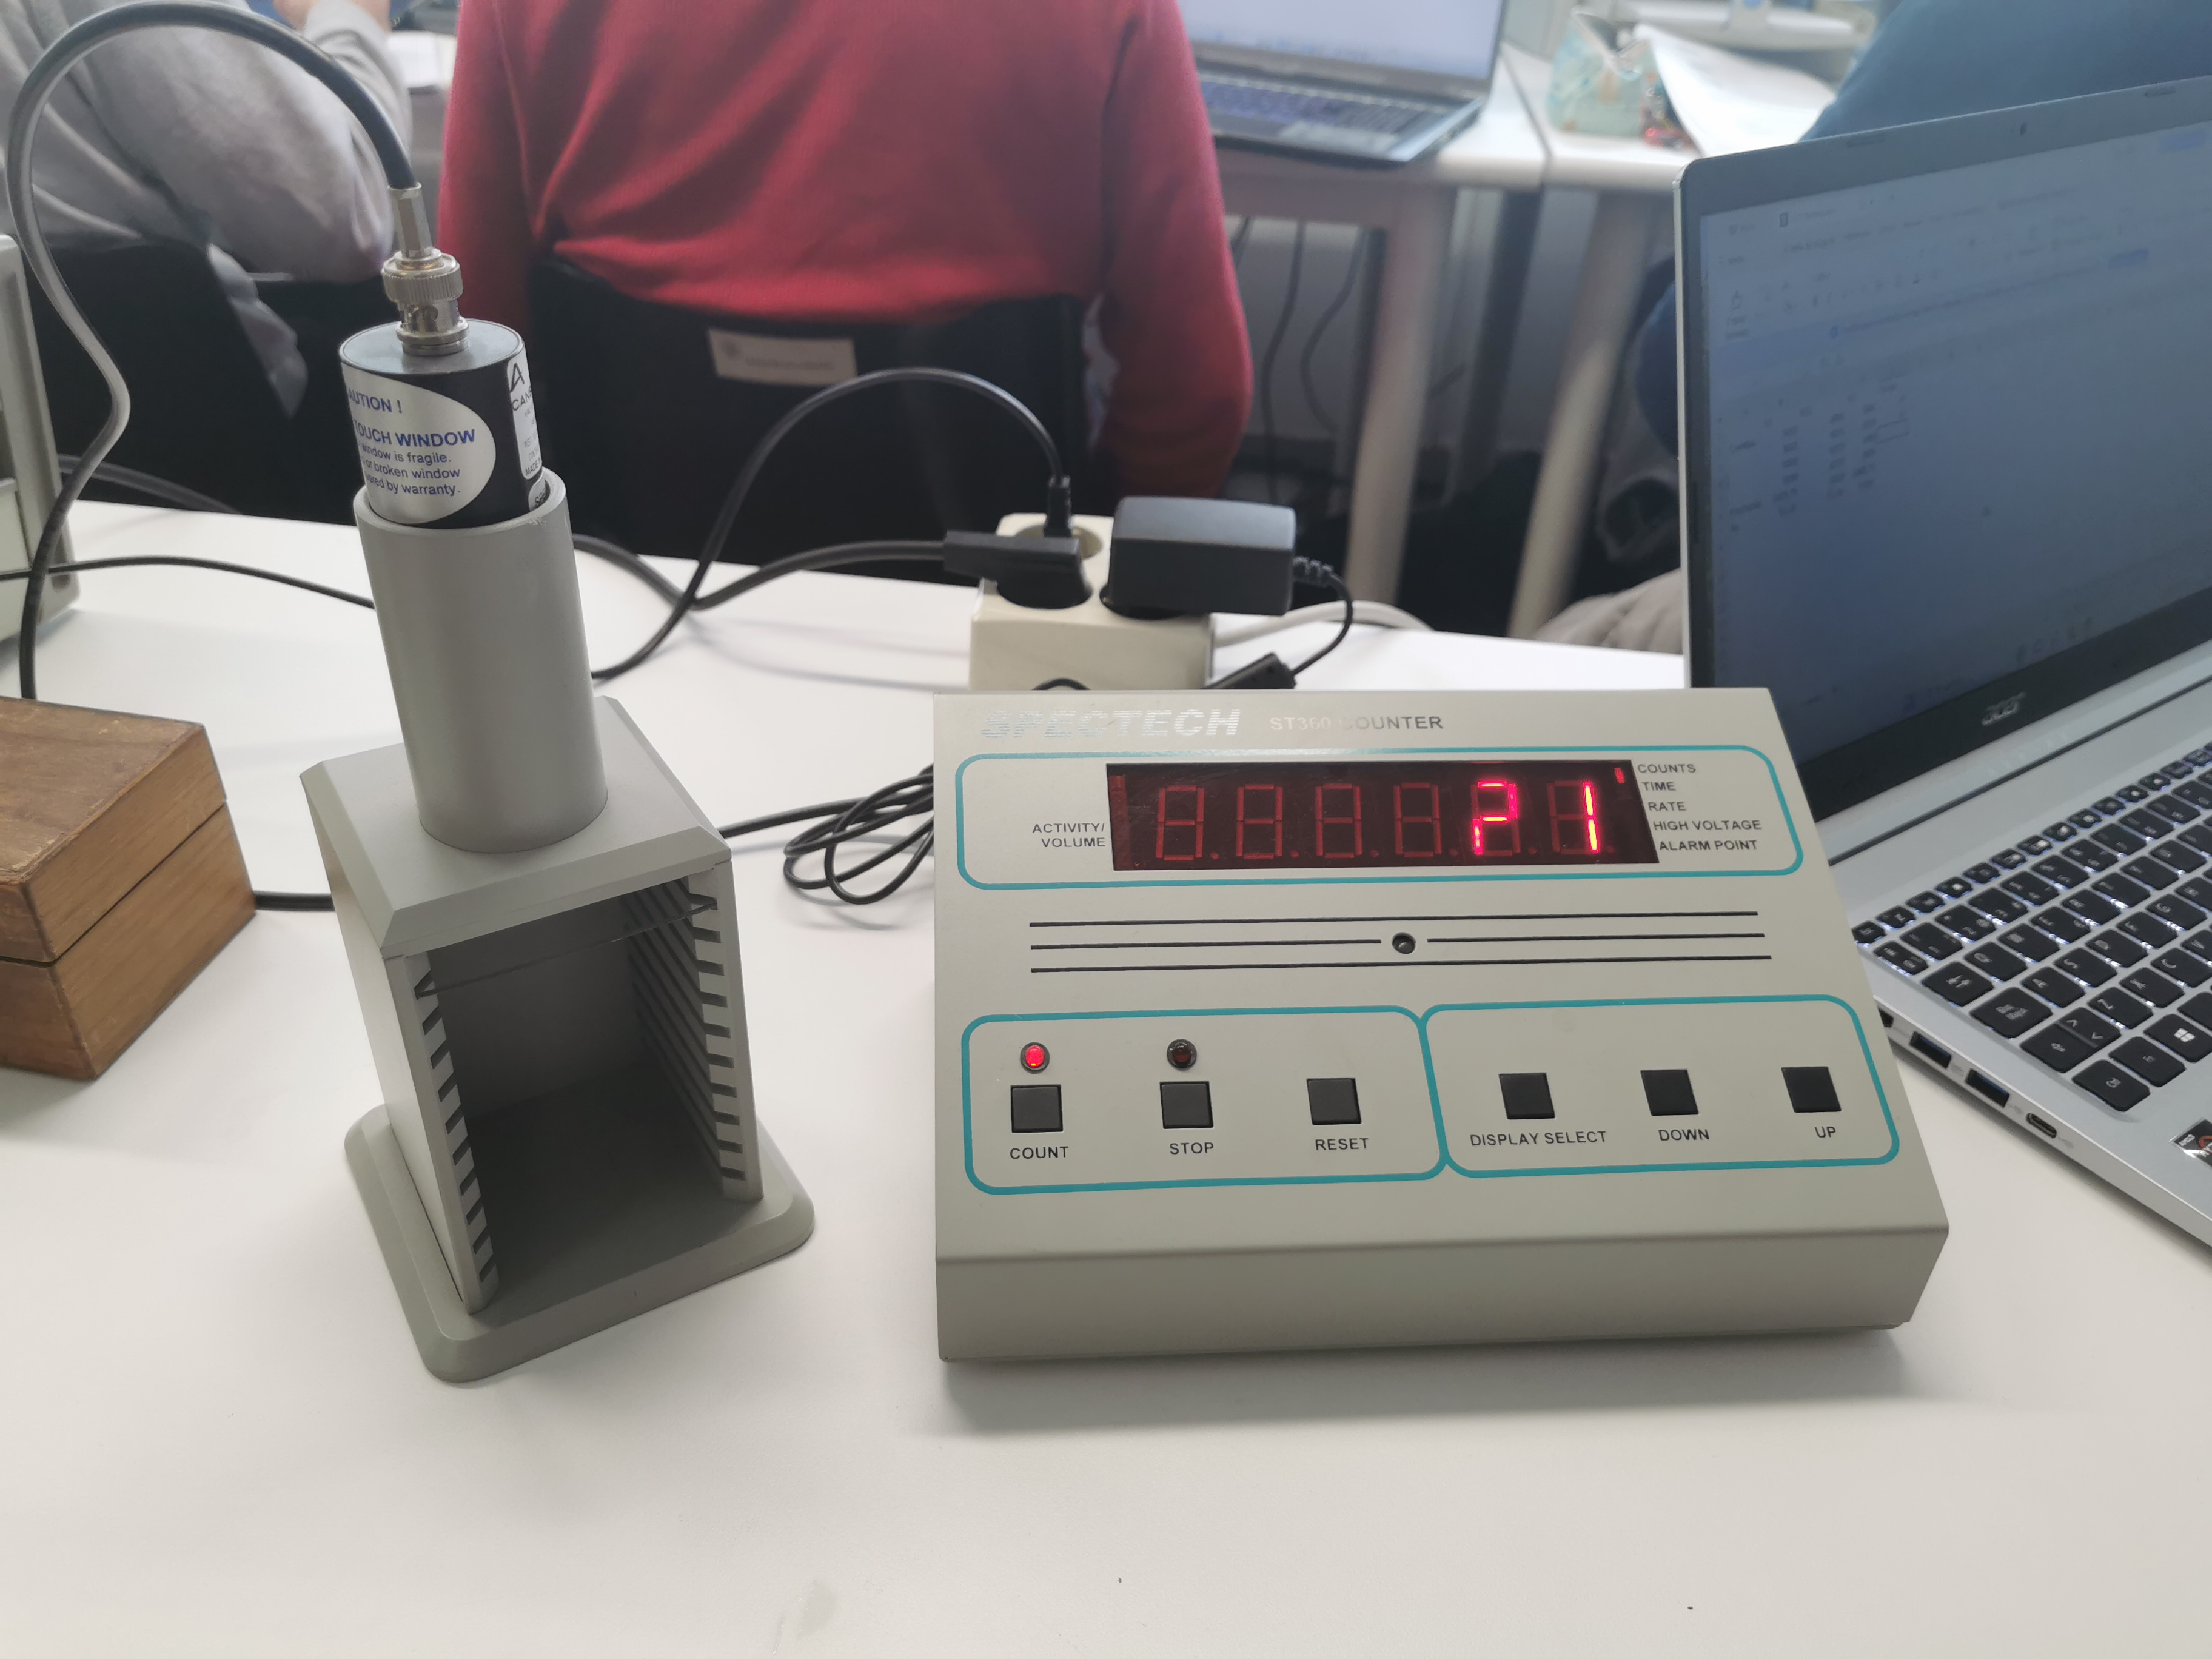
\includegraphics[width=0.7\linewidth]{imagenes/detector}
		\caption{Detector Geiger-Müller utilizado}
		\label{fig:detector}
	\end{figure}
	
	
	Teniendo en cuenta que seguimos tomando medidas de $t = 90\si{s}$
	
	\begin{table}[H]
		\centering
		\begin{tabular}{c|c|c|c|c|}
			\cline{2-5}
			& $A'_1$  & $A'_12$ & $A'_2$  & $F'$ \\ \hline
			\multicolumn{1}{|c|}{Cuentas 1} & 5037    & 6905    & 1892    & 47    \\ \hline
			\multicolumn{1}{|c|}{Cuentas 2} & 5022    & 6871    & 1839    & 67    \\ \hline
			\multicolumn{1}{|c|}{Cuentas 3} & 5070    & 6777    & 1883    & 59    \\ \hline
			\multicolumn{1}{|c|}{Cuentas 4} & 5094    & 6727    & 1909    & 43    \\ \hline\hline
			\multicolumn{1}{|c|}{Promedio}  & 5055,75 & 6820    & 1880,75 & 54    \\ \hline\hline
			\multicolumn{1}{|c|}{Bq}        & 56,18   & 75,78   & 20,90   & 0,60  \\ \hline
		\end{tabular}
		\caption{Medidas para el método de las dos fuentes}
		\label{tab:my-table}
	\end{table}
	
	
	Obtenemos un tiempo de resolución de
	
	\[ \tau_r = 0,000323 s = 323\si{\mu s}
	\]
	
	\section{Cálculo de la eficiencia}
	
	La eficiencia de un detector, $\varepsilon$, se puede definir como el cociente entre el las partículas detectadas y las partículas emitidas realmente por la fuente. El detector Geiger tiene una alta eficiencia  para detectar partículas $\alpha$ y $\beta$, pero para la radiación $\gamma$ es mucho menos eficiente.
	
	
	Para calcular la eficiencia, tomaremos la medida de la emisión de la muestra en un tiempo, corregiremos el fondo, y lo compararemos con la actividad real corrigiendo por su desintegración en la fecha medida:
	\[ A = A_0  e^{-\lambda t}
	\]
	
	
	
	
	
	
	
	
	\subsection*{Cobalto-60} % fuente de beta también?
	
	
		
	\begin{itemize}
		\item Tiempo de medida: $t = 90\si{s}$
		\item Número de cuentas: $L = 5410$ 
		\item Fondo: $F = 54$
		\item Tasa de recuento neta: $A' = \frac{(L- F)}{t} = 59,51\si{Bq} $
		\item Actividad inicial: $A_0 = 1\si{\mu Ci}$
		\item Fecha: 3/11/2022
		\item Periodo: $T_{1/2} = 5,26$ años
		\item Actividad corregida: $A = 31397,3\si{Bq}$ 
		\item Eficiencia: $\varepsilon = \frac{A'}{A} = 0,0020 \longrightarrow \varepsilon = 0,2\%$  
	\end{itemize}
	
	\subsection*{Estroncio-90}  % fuente de partículas beta
	
	
	
	\begin{itemize}
		\item Tiempo de medida: $t = 90\si{s}$
		\item Número de cuentas: $L = 20412$ 
		\item Fondo: $F = 54$
		\item Tasa de recuento neta: $A' = \frac{(L- F)}{t} = 226,2\si{Bq} $
		\item Actividad inicial: $A_0 = 0,1\si{\mu Ci}$
		\item Fecha: 02/2015
		\item Periodo: $T_{1/2} = 28,1$ años
		\item Actividad corregida: $A = 2957,4\si{Bq}$ 
		\item Eficiencia: $\varepsilon = \frac{A'}{A} = 0,0765 \longrightarrow \varepsilon = 7,65\%$  
	\end{itemize}
	
	\textit{Nota: los cálculos fueron realizados el 4/03/2024}\\
	
	Podemos ver que hay una diferencia significativa en la eficiencia del detector para ambos casos, un orden de magnitud de diferencia. El motivo de esto es la diferencia en las emisiones de cada material, y el modo en que esta emisión es detectada. El detector Geiger-Müller es relativamente bueno detectando partículas beta de alta energía, pero es peor con las de baja energía por la atenuación que ofrece el material que lo rodea, y la inherente a este. \\
	
	La eficacia del recuento de radiación gamma depende de la eficiencia de la interacción de la radiación con la pared del tubo, que aumenta con el número atómico del material de la pared. Comunmente se usa hierro cromado, que suele ofrecer una eficiencia en torno al 1\%.\\
	
	El detector puede saturarse con altas tasas de recuento de radiación, ya que se generan muchos electrones libres en rápida sucesión dentro del detector, lo que produce pulsos demasiado pequeños que el sistema electrónico no detecta. Esto provoca situaciones en las que las medidas muestran lecturas muy bajas de radiación en situaciones en las que hay mucha.\\
	
	La eficiencia también puede verse afectada por la distancia de las muestras (por la atenuación del aire), el tipo de pantalla, y la geometría de la muestra como indicamos anteriormente.\\
	
	En vista de los resultados obtenidos, el Cobalto-60 está produciendo una saturación sobre el detector, por sus altas emisiones de partículas gamma.  El Estroncio-90 en cambio tiene una eficiencia razonable, debido a que este detector está mucho mejor preparado para detectar las partículas beta que emite.
	
	
	
	
	
\end{document}